Mitä on web-palvelut?

Arkkitehtuureja? MVC? Komponentit?

Käyttäjädatan tallennus
- passwd (ts tiedosto levyllä tms)
- tietokanta
- AD-kannat (LDAP)

---> käyttäjän datan abstraktoinnin tarve, ehkä mainita, että käyttäjädatan backendejä voi käytännössä olla monta erilaista. Esim. LDAP:n rinnalla tietokannat.

Tunnistautumiseen liittyvien käsitteiden läpikäynti ennen protokollien yksityiskohtaista esittelyä auttaa tunnistautumiseen liittyvien periaatteiden hahmottamista. Käsitteet ovat yleisluontoisia ja eivätkä kosketa vain tiettyjä protokollaa. Protokollien yhteydessä käytetään käsitteitä asiakasohjelma, tunnistautumispalvelu, suojattu resurssi, valtuutustieto (credentials), valtuutusavain (authorization code) ja pääsyvaltuutus (access token) \cite{nisti}.

Asiakasohjelmalla tarkoitetaan web-palvelun käyttäjän pääteohjelmaa, jolla hän kirjautuu web-palveluun käyttäen keskitettyä tunnistautumispalvelua. Käytännössä asiakasohjelma on web-palvelun tapauksessa käyttäjän WWW-selain, joka pystyy tekemään uudelleenohjauksia sivustolta toiselle. Uudelleenohjaus on HTTP-protokollan perustoiminnallisuutta, joten mikä tahansa HTTP/1.1-standardin WWW-selain käy asiakasohjelmaksi \cite{rfc2616}.

Tunnistautumispalvelu on web-palvelu, johon käyttäjä ohjataan tekemään tunnistautuminen. Onnistuneen tunnistautumisen jälkeen tunnistautumispalvelu ohjaa asi\-a\-kas\-oh\-jel\-man takaisin tunnistautumista pyytäneen palvelun määrittelemään osoitteeseen \cite{nisti}. Avoimen Internetin puolella tunnistautumispalvelu voi olla esimerkiksi Facebook tai LinkedIn.

Tunnistautumisprotokollien yhteydessä suojatulla resurssilla tarkoitetaan resurssia, jonka käyttö vaatii tunnistautumisen ja käyttöoikeuden. Yleisessä tapauksessa suojatulla resurssilla tarkoitetaan yksittäistä resurssia (käyttäjän valokuvaa), johon halutaan asettaa pääsyrajoituksia \cite{nisti}. Tämän tutkielman puitteissa suojatulla resurssilla tarkoitetaan tunnistautumista vaativaa web-palvelua.

Valtuutustieto koostuu yksilöivästä tunnisteesta ja siihen liittyvästä salaisesta avaimesta. Tämän tutkielman puitteissa valtuutustiedolla tarkoitetaan käyttäjän tunnusta ja salasanaa.

Kirjauduttuaan sisään tunnistautumispalvelimelle, käyttäjä saa valtuutusavaimen, jonka hän lähettää eteenpäin suojatun resurssin omistajalle. Valtuutusavain ei pidä sisällään käyttäjän valtuutustietoja, vaan ainoastaan tunnistautumispalvelin osaa lukea sen \cite{nisti}. Saatuaan valtuutusavaimen käyttäjältä voi suojatun resurssin omistaja hakea pääsyvaltuuden käyttäjän tietoihin tunnistautumispalvelusta.

Pääsyvaltuutus on tunnistautumispalvelimelta saatava yksilöivä tunniste, jonka avulla suojatun resurssin omistaja voi pyytää käyttäjän tiedot tunnistautumispalvelulta. Pääsyvaltuutus on voimassa tietyn ajan, jonka jälkeen se täytyy uusia tunnistautumispalvelimella \cite{nisti}. Pääsyvaltuutusta voidaan käyttää myös tunnistautumispalvelusta erillään olevien resurssien valtuuttamiseen. Esimerkiksi web-sovellus voi hakea tunnistautumispalvelulta pääsyvaltuuden, jolla hän hakee valokuvia valokuvien jakopalvelusta \cite{facebook}.
\subsection{Arkkitehtuurit}
Servlet- tai FastCGI-tekniikka ei sido web-sovelluksen arkkitehtuuria, vaan molempia tekniikoita käytettäessä sovellusten perusarkkitehtuuri on sama. Sovellukset ovat jatkuvasti pyöriviä prosesseja, jotka saavat syötteenään käyttäjän syöttämän datan lisäksi joukon erilaisia suoritusympäristöön liittyviä resursseja ja muuttujia (mm. tietokantayhteys) \cite{uml}. Syötteen perusteella sovellus tuottaa tulosteen, joka palautetaan käyttäjälle.

Tyypillinen tapa toteuttaa web-sovelluksia nykypäivänä on käyttää sovelluskehystä, mikä tuo oman lisänsä sovellusten arkkitehtuuriin. Käytettyjä kehyksiä on esimerkiksi Javalla toteutettu Spring, Pythonin Django ja Ruby-ohjelmointikieleen luottava Ruby on Rails \cite{spring, django, ruby2011agile}. Näissä sovelluskehyksissä erillinen viestinvälittäjä (dispatcher) ottaa vastaan pyynnön ja välittää sen eteenpäin sovellusohjelmalle. Pyyntö ei siirry suoraan sovellusohjelmalle, vaan se välitetään väliohjelma-kerroksen läpi kuvassa \ref{dispatcher} esitetyllä tavalla. Nämä väliohjelmat esimerkiksi tekevät merkintöjä lokitiedostoihin, asettavat ja lukevat käyttäjän selaimen evästeitä tai asettavat ympäristömuuttujia sovellusohjelmaa varten.

\begin{figure}[ht]
\centering
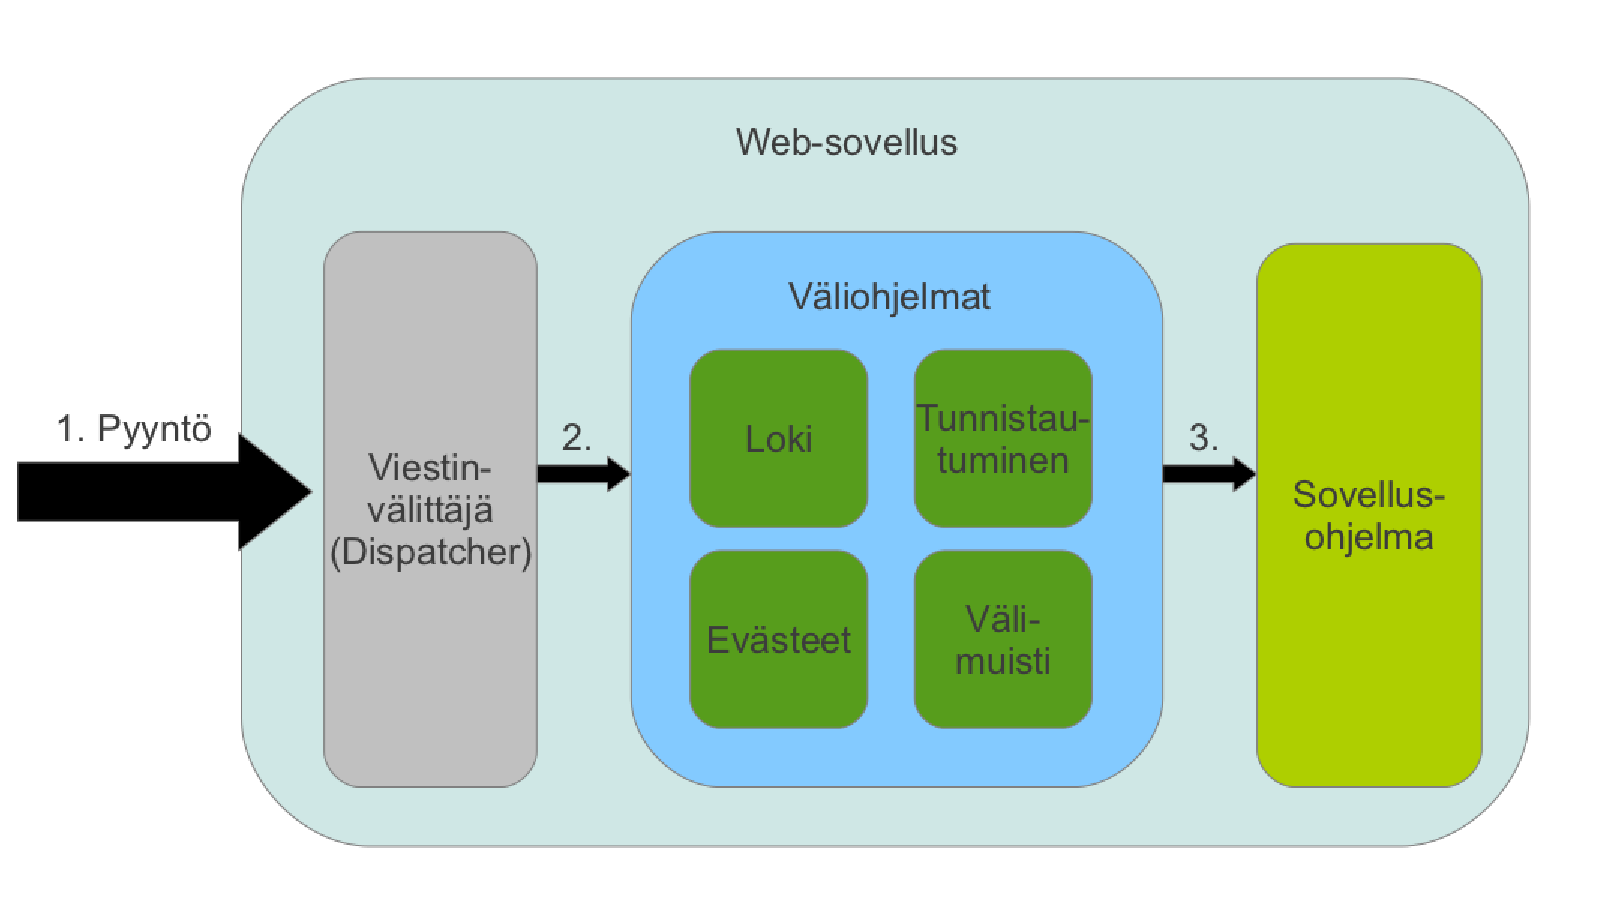
\includegraphics[width=\textwidth]{web/dispatcher.eps}
\caption{Web-sovelluskehyksellä toteutetun web-sovelluksen kontrollin kulku \cite{ruby2011agile}.}%
\label{dispatcher}
\end{figure}

Sovellusohjelmasta on pyritty karsimaan paljon yleisiä tehtäviä sovelluskehyksen tai käyttäjän toteuttaman väliohjelman tehtäväksi. Web-sovellus käyttää hyväkseen sovelluskehyksen tarjoamia parametreja, jotka ovat esimerkiksi viittauksia muuttujiin, joita säilytetään käyttäjän istunnon ajan muistissa. Myös käyttäjän tunnistautuminen on yksi sovelluskehyksen tehtävistä \cite{ruby2011agile}. Tällöin sovellusohjelma saa ympäristömuuttujana kirjautuneen käyttäjän tiedot (esimerkiksi tunnistenumeron ja käyttöoikeudet), joita se käyttää hyväksi ohjelmalogiikassaan.

CGI-ohjelmien tietovuopohjaisesta arkkitehtuurityylistä on sovelluskehysten myötä menty modulaarisiin arkkitehtuureihin. Saman sovelluskehyksen sisällä voi olla useampia ohjelmamoduuleita, joita viestinvälittäjä kutsuu esimerkiksi URL-osoitteen perusteella. Kun ohjelmamoduuleiden ei tarvitse toteuttaa kaikkea perustoiminallisuutta itse, yksinkertaistuu niiden rakenne. Web-sivustot saattavat käyttää hyväksi myös useampaa yksittäistä web-sovellusta, jolloin puhutaan palveluperustaisista arkkitehtuureista.
\subsection{Käyttäjädata}
Tunnistautumiseen liittyvien käsitteiden läpikäynti ennen protokollien yksityiskohtaista esittelyä auttaa tunnistautumiseen liittyvien periaatteiden hahmottamista. Käsitteet ovat yleisluontoisia ja eivätkä kosketa vain tiettyjä protokollaa. Protokollien yhteydessä käytetään käsitteitä asiakasohjelma, tunnistautumispalvelu, suojattu resurssi, valtuutustieto (credentials), valtuutusavain (authorization code) ja pääsyvaltuutus (access token) \cite{nisti}.

Asiakasohjelmalla tarkoitetaan web-palvelun käyttäjän pääteohjelmaa, jolla hän kirjautuu web-palveluun käyttäen keskitettyä tunnistautumispalvelua. Käytännössä asiakasohjelma on web-palvelun tapauksessa käyttäjän WWW-selain, joka pystyy tekemään uudelleenohjauksia sivustolta toiselle. Uudelleenohjaus on HTTP-protokollan perustoiminnallisuutta, joten mikä tahansa HTTP/1.1-standardin WWW-selain käy asiakasohjelmaksi \cite{rfc2616}.

Tunnistautumispalvelu on web-palvelu, johon käyttäjä ohjataan tekemään tunnistautuminen. Onnistuneen tunnistautumisen jälkeen tunnistautumispalvelu ohjaa asi\-a\-kas\-oh\-jel\-man takaisin tunnistautumista pyytäneen palvelun määrittelemään osoitteeseen \cite{nisti}. Avoimen Internetin puolella tunnistautumispalvelu voi olla esimerkiksi Facebook tai LinkedIn.

Tunnistautumisprotokollien yhteydessä suojatulla resurssilla tarkoitetaan resurssia, jonka käyttö vaatii tunnistautumisen ja käyttöoikeuden. Yleisessä tapauksessa suojatulla resurssilla tarkoitetaan yksittäistä resurssia (käyttäjän valokuvaa), johon halutaan asettaa pääsyrajoituksia \cite{nisti}. Tämän tutkielman puitteissa suojatulla resurssilla tarkoitetaan tunnistautumista vaativaa web-palvelua.

Valtuutustieto koostuu yksilöivästä tunnisteesta ja siihen liittyvästä salaisesta avaimesta. Tämän tutkielman puitteissa valtuutustiedolla tarkoitetaan käyttäjän tunnusta ja salasanaa.

Kirjauduttuaan sisään tunnistautumispalvelimelle, käyttäjä saa valtuutusavaimen, jonka hän lähettää eteenpäin suojatun resurssin omistajalle. Valtuutusavain ei pidä sisällään käyttäjän valtuutustietoja, vaan ainoastaan tunnistautumispalvelin osaa lukea sen \cite{nisti}. Saatuaan valtuutusavaimen käyttäjältä voi suojatun resurssin omistaja hakea pääsyvaltuuden käyttäjän tietoihin tunnistautumispalvelusta.

Pääsyvaltuutus on tunnistautumispalvelimelta saatava yksilöivä tunniste, jonka avulla suojatun resurssin omistaja voi pyytää käyttäjän tiedot tunnistautumispalvelulta. Pääsyvaltuutus on voimassa tietyn ajan, jonka jälkeen se täytyy uusia tunnistautumispalvelimella \cite{nisti}. Pääsyvaltuutusta voidaan käyttää myös tunnistautumispalvelusta erillään olevien resurssien valtuuttamiseen. Esimerkiksi web-sovellus voi hakea tunnistautumispalvelulta pääsyvaltuuden, jolla hän hakee valokuvia valokuvien jakopalvelusta \cite{facebook}.
\subsubsection{passwd}
Vanha kunnon /etc/passwd, tästä tunnistautuminen on varmaan lähtenyt käyntiin. Ikävää, kun webiin tunnistautuessa täytyy olla tunnus kyseisellä koneella ja muutenkin ei ole hyvä kun tunnukset siirtyy verkkoa pitkin.
\subsubsection{Relaatiotietokannat}
Käyttäjätietokannat, relaatiokannat lähinnä, ehkä NoSQL.
\subsubsection{LDAP}
Lähteet: Howes, T. A., The Lightweight Directory Access Protocol: X.500 Lite. CITI
Technical Report 95–8, University of Michigan, 1995. \cite{howes} \\
rfc:t 4510-4513 (ainakin 4513 "Authentication Methods and Security Mechanisms" kiinnostaa)

Lightweight Directory Access Protocol (LDAP) on X.500 OSI-standardiin perustuva hakemistopalvelu, jota käytetään yleisesti käyttäjätiedon tallennukseen [TODO: lähde]. 1990-luvulla TCP/IP-mallin syrjäytettyä OSI-mallin, myös DAP kävi vanhanaikaiseksi \cite{howes}. Korvaajaksi on noussut LDAP, josta käytetään myös nimeä X.500 Lite \cite{howes}.

LDAP:ssa asiakassovellukset (directory user agent, DUA) keskustelevat puumalliin perustuvan hakemistopalvelimen (directory system agent, DSA) kanssa käyttäen määriteltyä protokollaa (directory access protocol, DAP) \cite{howes}. Asiakassovellukset voivat hakea hakemistopalvelimesta tietoa suodattimiin (filter) perustuvalla lukuoperaatiolla. Suodattimessa voidaan määritellä raja-arvot attribuutin arvolle tai hakea avainsanoilla attribuuteista.

LDAP-tietuille voidaan määritellä pakollisten attribuuttien (esim. etu- ja sukunimi) lisäksi valinnaisia attribuutteja. Tietueet on järjestetty puuhun niiden yksilöivän nimen (distinguished name, DN) mukaan ja ne voi olla hajautettu usealle palvelimelle. Suhteellinen nimi (relative distinguished name, RDN) identifioi tietueen omalla hierarkiatasollaan.

LDAP-tietueella voi olla tunnus sekä salasana ja LDAP-palvelinta voidaan käyttää käyttäjän tunnistautumiseen [TODO: lähde, ehkä rfc4513].

TODO: lisää tekstiä

\subsubsection{Käyttäjädatan abstraktointi}
Tutkimuksen kannalta abstraktointi on oleellista, oikeastaan sillä ei ole ison kuvan kannalta merkitystä, että onko siellä taustalla tietokanta, tiedosto, ldap vai mikä.
\subsection{Yhteenveto}
Käytetään OAuthia protossa, koska OpenID:ssä kaikkea tarpeetonta mukana. SAML taas skipataan, koska...? Tätä pitäisi pohtia jossain kohtaa.